% 對應英文：sections/07_results.tex

\section{主要結果}

表~\ref{tab:cross_model} 呈現所有（模型、特徵組合）
在留出測試集（第 275--323 週，共 49 週）上的年化夏普比率。
橫列代表資訊集的逐步擴充，
直欄則比較三種深度學習架構與六個傳統基準模型在等權（EW）與市值加權（PW）下的表現。

% Auto-generated by gen_tables.py -- do not edit manually
\begin{table*}[t]
\centering
\caption{Cross-model comparison: annualised Sharpe ratios on the test set. The held-out period contains 49 panel weeks; after masking, portfolio metrics use 48 valid weekly long-short returns.}
\label{tab:cross_model}
\begingroup
\footnotesize
\setlength{\tabcolsep}{3pt}
\begin{tabular}{@{}lrrrrrrrrr@{}}
\toprule
\thead{Information Set} & \thead{CS\_Gated} & \thead{LSTM} & \thead{TFT} & \thead{OLS} & \thead{ElasticNet} & \thead{PCA} & \thead{PLS} & \thead{RF} & \thead{GBT} \\
\midrule
\multicolumn{10}{l}{\textit{Panel A: Equal-Weight (EW)}} \\
\midrule
Price{+}Technical & 1.344 & 1.447 & 0.116 & 1.208 & 1.275 & 0.391 & 0.642 & 1.218 & \textbf{1.737} \\
{+}Onchain & \textbf{2.753$^\dagger$} & 1.128 & 1.319 & 1.085 & 1.275 & 0.421 & 0.624 & 1.554 & 1.623 \\
All & 0.856 & 0.366 & 0.442 & 1.194 & 1.275 & 0.457 & 0.624 & \textbf{2.098} & -0.009 \\
{+}Trump & 1.242 & 0.588 & 0.930 & 1.289 & 1.093 & 0.375 & 0.828 & \textbf{1.983} & 1.147 \\
{+}ETF & \textbf{1.421} & 0.574 & 0.885 & 1.194 & 1.275 & 0.457 & 0.624 & 1.272 & -0.009 \\
{+}Trump{+}ETF & 1.824 & \textbf{2.033$^\dagger$} & 1.761 & 1.310 & 1.093 & 0.375 & 0.828 & 1.475 & 1.147 \\
\midrule
\multicolumn{10}{l}{\textit{Panel B: Price-Weighted (PW)}} \\
\midrule
Price{+}Technical & 1.333 & \textbf{2.453$^\dagger$} & 0.135 & 1.130 & 1.275 & 0.434 & 0.578 & 1.289 & 1.563 \\
{+}Onchain & \textbf{2.607$^\dagger$} & 0.932 & 1.059 & 1.003 & 1.275 & 0.464 & 0.870 & 1.471 & 1.434 \\
All & 1.252 & 0.591 & 0.165 & 1.244 & 1.275 & 0.564 & 0.725 & \textbf{1.572$^\dagger$} & 0.998 \\
{+}Trump & 0.895 & 0.566 & 0.977 & 1.314 & 1.028 & 0.409 & 0.815 & \textbf{1.620} & 1.235 \\
{+}ETF & 1.157 & 0.356 & 0.867 & 0.932 & 1.275 & 0.565 & 1.026 & \textbf{1.431} & 0.998 \\
{+}Trump{+}ETF & 1.613 & \textbf{2.135$^\dagger$} & 1.869$^\dagger$ & 1.203 & 1.029 & 0.410 & 0.815 & 1.398 & 1.235 \\
\bottomrule
\end{tabular}
\endgroup
\par\vspace{0.35em}
\begin{minipage}{0.96\linewidth}
\raggedright\footnotesize
\textit{Note:} $\dagger$ indicates that the 95\% circular block-bootstrap confidence interval for the annualised Sharpe ratio excludes zero. Bootstrap block length is $b=\max(2,\lfloor T^{1/3}\rfloor)$. Bold entries mark the best model within each information set and weighting scheme.
\end{minipage}
\end{table*}


\paragraph{橫截面門控網路（CS-Gated）。}
CS-Gated 在「+鏈上」組合下取得整體最佳表現，
等權夏普比率為 2.75、市值加權為 2.61。
這一結果的重要意義在於，
當輸入主要是 NVT、MVRV、交易所淨流量等較為結構性的當期特徵時，
純橫截面模型並不會因缺乏時序編碼而吃虧。
相反地，GRN 與跨資產注意力足以從同一週的相對位置中學出可交易的排序規則。
然而，CS-Gated 在加入「+川普+ETF」後並未進一步受益，
等權夏普比率自 2.75 降至 1.82，
顯示事件性較強、時間相依較高的替代資料，
未必適合用純當期快照的方式處理。

\paragraph{LSTM。}
LSTM 的最佳設定出現在「+川普+ETF」，
市值加權夏普比率為 2.13、等權為 2.03，
是時序模型中最穩健的表現。
與 CS-Gated 不同，LSTM 在納入川普社群媒體與 ETF 結構流量後明顯改善，
顯示其時序編碼器能捕捉單週快照看不見的序列關係，
例如政策發文的聚集、資金流的延續性，或事件後數週的市場消化過程。
值得注意的是，LSTM 在「全部」組合的表現反而偏弱，
說明並非特徵越多越好；
若資料中混入不同預測頻率與不同噪音結構的訊號，
模型反而可能難以形成穩定的排序規則。

\paragraph{時序融合轉換器（TFT）。}
TFT 在小型資訊集上的表現不如 LSTM，
例如「價格+技術指標」下的等權夏普僅 0.12，
顯示較高容量的架構在簡單特徵集上容易訓練不穩。
然而，當加入「+川普+ETF」後，
TFT 的市值加權夏普上升至 1.87、等權為 1.76，
改善幅度與 LSTM 類似。
這代表 TFT 並非無法利用替代資料，
而是更依賴完整且具資訊密度的特徵組合，才能讓 VSN 與注意力機制發揮作用。
相較於 LSTM，TFT 的優勢較偏向可解釋性；
其弱點則是每種子結果較不穩定，後續在第~\ref{sec:analysis:ensemble}~節中也會看到這一點。

\paragraph{傳統基準模型。}
傳統模型在本研究中並非容易被深度學習全面壓制的弱基準。
隨機森林（RF）在「全部」組合下達到等權夏普 2.10，
甚至優於同列的三種深度學習模型；
在「+川普」下，RF 的等權夏普亦達 1.98，仍具強勁競爭力。
這表示當特徵維度提高且非線性交互作用複雜時，
樹模型能夠在不承受神經網路訓練不穩定性的情況下，有效擷取可交易訊號。
相較之下，OLS 與 ElasticNet 的表現雖不差，
但大致維持在約 1.0 至 1.3 的區間，
說明線性模型具備穩定性，卻較難把不同來源特徵之間的非線性交互作用轉化為更高 Sharpe。

\paragraph{整體比較與研究意涵。}
綜合而言，本文結果並不支持「單一架構在所有資料型態下全面勝出」的說法。
真正的結論是：模型優勢取決於它所面對的訊號結構。
當主要訊號來自較慢變、可直接做橫截面比較的鏈上基本面時，
CS-Gated 最具優勢；
當訊號包含具有延續性的社群媒體與 ETF 流量時，
LSTM 與 TFT 的時序能力便開始發揮價值；
當特徵維度較高且交互關係複雜時，
RF 仍是不可忽視的強勁對手。
因此，本文的核心發現並非「深度學習必然優於傳統方法」，
而是「在正確的排序損失與適配的資料組合下，不同模型會對不同訊號型態展現專長」。

\section{累積報酬}

\begin{figure}[t]
  \centering
  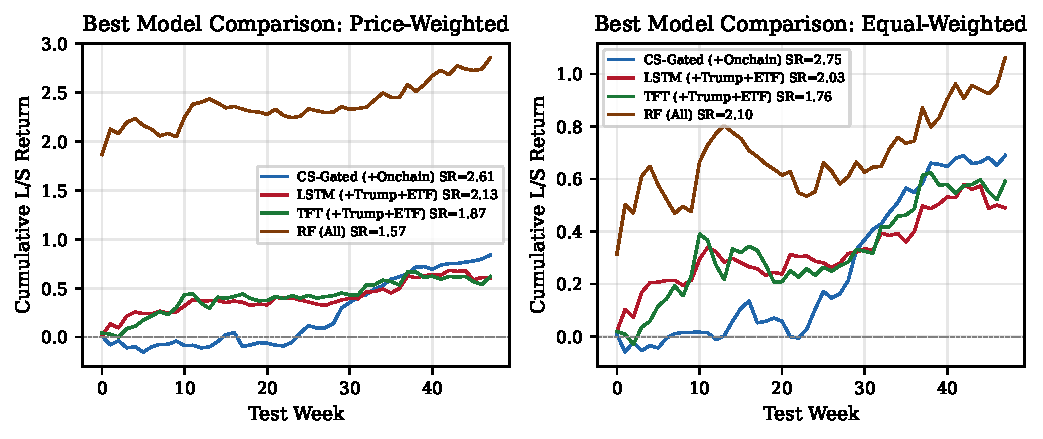
\includegraphics[width=\linewidth]{figures/cum_returns_combined.pdf}
  \caption{各模型最佳設定的多空累積報酬曲線：
           CS-Gated（\texttt{+鏈上}）、LSTM（\texttt{+川普+ETF}）、
           TFT（\texttt{+川普+ETF}）與 RF（\texttt{全部}），
           並以等權市場投資組合作為對照。
           圖例中的 CR（cumulative return）為各策略的期末累積報酬，
           即曲線終點值，屬報酬「規模」指標，
           並非圖~\ref{fig:sr_combined_zh} 的風險調整夏普比率。}
  \label{fig:cumret_combined_zh}
\end{figure}

圖~\ref{fig:cumret_combined_zh} 顯示，
最佳模型的累積報酬並非由單一極端週次所驅動，
而是在測試期間中逐步累積出差異。
其中，CS-Gated 與 LSTM 的曲線最為陡峭，
但兩者的資料依賴來源不同：
前者主要來自鏈上基本面排序的穩定性，
後者則更像是對政策與資金流事件的時序回應。
RF 雖在部分資訊集上具競爭力，
其累積報酬斜率相對較不穩定，與其在不同資訊集間表現起伏較大的現象一致。

\begin{figure}[t]
  \centering
  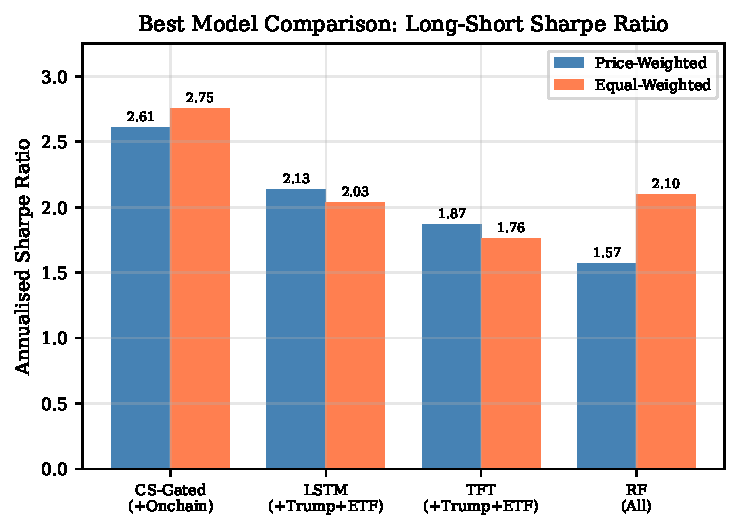
\includegraphics[width=0.8\linewidth]{figures/sr_comparison.pdf}
  \caption{各模型最佳設定的多空年化夏普比率：
           CS-Gated（\texttt{+鏈上}）、LSTM（\texttt{+川普+ETF}）、
           TFT（\texttt{+川普+ETF}）與 RF（\texttt{全部}），
           分別以價格加權與等權建構。與圖~\ref{fig:cumret_combined_zh}
           所繪的期末累積報酬不同，本圖呈現的是風險調整後的績效。}
  \label{fig:sr_combined_zh}
\end{figure}

圖~\ref{fig:sr_combined_zh} 以風險調整角度重述同一組比較。
CS-Gated（\texttt{+鏈上}）在兩種加權方式下皆取得最高夏普比率（價格加權 2.61、等權 2.75）；
反觀 RF 雖在圖~\ref{fig:cumret_combined_zh} 中累積報酬最高，
其價格加權夏普比率卻最低（1.57），原因在於其報酬幅度大但波動亦大。
兩張圖衡量的對象不同：累積報酬獎勵的是總幅度，
夏普比率獎勵的是穩定性，而表~\ref{tab:cross_model} 的模型排序正是依據後者。

\section{分位夏普比率}

\begin{figure}[t]
  \centering
  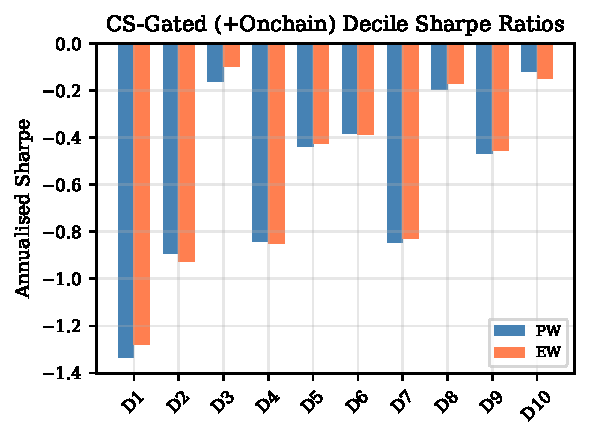
\includegraphics[width=\linewidth]{figures/decile_sharpe_cs_gated.pdf}
  \caption{CS-Gated（\texttt{+鏈上}）各預測分位投資組合的夏普比率。
           第 1 分位為最低預測排名（空頭端），第 10 分位為最高預測排名（多頭端）。
           柱狀圖同時呈現 PW 與 EW 投資組合。}
  \label{fig:decile_cs_gated_zh}
\end{figure}

圖~\ref{fig:decile_cs_gated_zh} 的分位夏普圖提供了另一種重要檢查：
圖中的柱狀值是各分位投資組合本身的夏普比率，
而表~\ref{tab:cross_model} 回報的是第 10 分位減第 1 分位的多空夏普比率；
兩者衡量的投資組合不同，因此排序不必完全一致。
在本研究的測試期間，多數單一分位投資組合的夏普比率為負，
中間分位也較為雜訊化。
較重要的訊號是最低預測分位明顯弱於最高預測分位，
代表模型仍捕捉到可用的橫斷面分離能力，
只是不能將其解讀為每個中間分位都具備平滑且單調的排序校準。
